\lstinputlisting[language=bash,basicstyle=\small]{python_codes/fieldstone_03/keywords}

\begin{center}
Code at \url{https://github.com/cedrict/fieldstone/tree/master/python_codes/fieldstone_03}
\end{center}

\par\noindent\rule{\textwidth}{0.4pt}
%%%%%%%%%%%%%%%%%%%%%%%%%%%%%%%%%%%%%%%%%%%%%%%%%%%%%%%%%%%%%%%%%%%%%%%%%%%%%%%%%%%%%%%%%

This benchmark deals with the 2-D thermal convection of a fluid 
of infinite Prandtl number in a rectangular closed cell.
In what follows, I carry out the case 1a, 1b, and 1c experiments as shown in 
Blankenbach \etal (1989) \cite{blbc89}:
steady convection with constant viscosity in a square box.

The temperature is fixed to zero on top and to $\Delta T$ at the bottom, 
with reflecting symmetry at the sidewalls (i.e. $\partial_x T=0$) 
and there are no internal heat sources. 
Free-slip conditions are implemented on all boundaries. 

The Rayleigh number is given by
\begin{equation}
\Ranb = \frac{\alpha g_y \Delta T h^3 }{\kappa \nu}
=\frac{\alpha g_y \Delta T h^3 \rho^2 C_p}{k \eta}
\end{equation}

In what follows, I use the following parameter values:  %, as given in \cite{krhb12}:
$L_x=L_y=1$,$\rho_0=c_P=k=\eta=1$, $T_0=0$, $\alpha=10^{-2}$, $g=10^{2}Ra$
and I run the model with $Ra=10^4,10^{5}$ and $10^6$.

The initial temperature field is given by 
\begin{equation}
T(x,y)=(1-y) - 0.01\cos(\pi x) \sin(\pi y)
\end{equation}
The perturbation in the initial temperature fields leads to 
a perturbation of the density field and sets the fluid in motion. 
Depending on the initial Rayleigh number, the system ultimately reaches a 
steady state after some time. 

The Nusselt number (i.e. the mean surface temperature gradient over mean bottom temperature)
is computed as follows \cite{blbc89}:
\begin{equation}
\Nunb = L_y \frac{\int_0^{L_x} \frac{\partial T}{\partial y}(y=L_y) \; dx  }{\int_0^{L_x} T(y=0) \; dx}
\label{eqNu}
\end{equation}
Note that in our case the denominator is equal to 1 since $L_x=1$ and the temperature at the 
bottom is prescribed to be 1.

If no convection is taking place (i.e. $\Ranb$ is too low) then only diffusion is taking place 
and the steady state temperature field is then $T(y)=1-y$, so that $\partial_y T=-1$ and 
we find that the Nusselt number is simply 1.

The steady state root mean square velocity and Nusselt number measurements
are indicated in the following Table alongside those of \cite{blbc89} and \cite{tack94}.
(Note that this benchmark was also carried out and published in  
other publications \cite{trha98,albe00,gery10,bepo10,dawk11,lezh11} but 
since they did not provide  a complete set
of measurement values, they are not included in the table.)

\begin{center}
\begin{tabular}{llcc}
\hline
          &           & Blankenbach et al (1989) & Tackley (1994) \cite{tack94}    \\
\hline
\hline
$\Ranb=10^4$ & $V_{rms}$ &  $42.864947  \pm 0.000020$ & 42.775 \\
          & $Nu$      &  $4.884409   \pm 0.000010$ & 4.878  \\
$\Ranb=10^5$ & $V_{rms}$ &  $193.21454  \pm 0.00010 $ & 193.11 \\
          & $Nu$      &  $10.534095  \pm 0.000010$ & 10.531 \\
$\Ranb=10^6$ & $V_{rms}$ &  $833.98977  \pm 0.00020 $ & 833.55 \\
          & $Nu$      &  $21.972465  \pm 0.000020$ & 21.998 \\
\hline
\end{tabular}\\
{\small Steady state Nusselt number $Nu$ and $\upnu_{rms}$ measurements as reported in the literature. }
\end{center}

Food for thought: Looking at the mass, momentum and energy conservation equations, 
we see that that they are coupled: the temperature enters the rhs of the momentum 
equation since the density depends on the temperature (Boussinesq approximation)
while the velocity is present in the advection term of the energy equation.
One should then solve all three equations with $u,v,p,T$ as unknowns. However
this is rarely done in practice and often the system is solved in a segregated way:
first solve for $u,v,p$ assuming $T$ known, then solving for $T$ assuming $u,v,p$ known.
If small time steps are used this is a reasonable approach, or, like in this case, when 
one wishes to compute the steady state of the system rather than an accurate time-evolution
of the system. Better schemes are available and one example thereof is explained in Kronbichler et al (2012) 
\cite{krhb12}.

Also, the current version of this stone uses a simple time discretisation of the $\partial T/\partial t$ term
as explained in Section~\ref{sec:diff1D}. A Crank-Nicolson algorithm could easily be 
implemented as explained in Section~\ref{sec:timediscr}.

Something must be said about how the Nusselt number is computed. 
Its calculation requires the integral of the temperature gradient along an edge. 
Because it is much simpler to compute the temperature gradient in the middle of the 
element alongside other quantities such as pressure, this (elemental) quantity is 
used in the Nusselt number calculations, which makes it inaccurate and therefore 
explains the discrepancy between the computed values and those of other publications.

Finally, it is expected that the thickness of the 
boundary layers decreases with higher Rayleigh number values.
As a consequence, in order to appropriately capture those, one needs 
a higher resolution than at low $\Ranb$ numbers. This explains why 
acceptable results are obtained for $\Ranb=10^4$  at low resolution 32x32.


\newpage
\paragraph{Results for $\Ranb=10^4$}.
\begin{center}
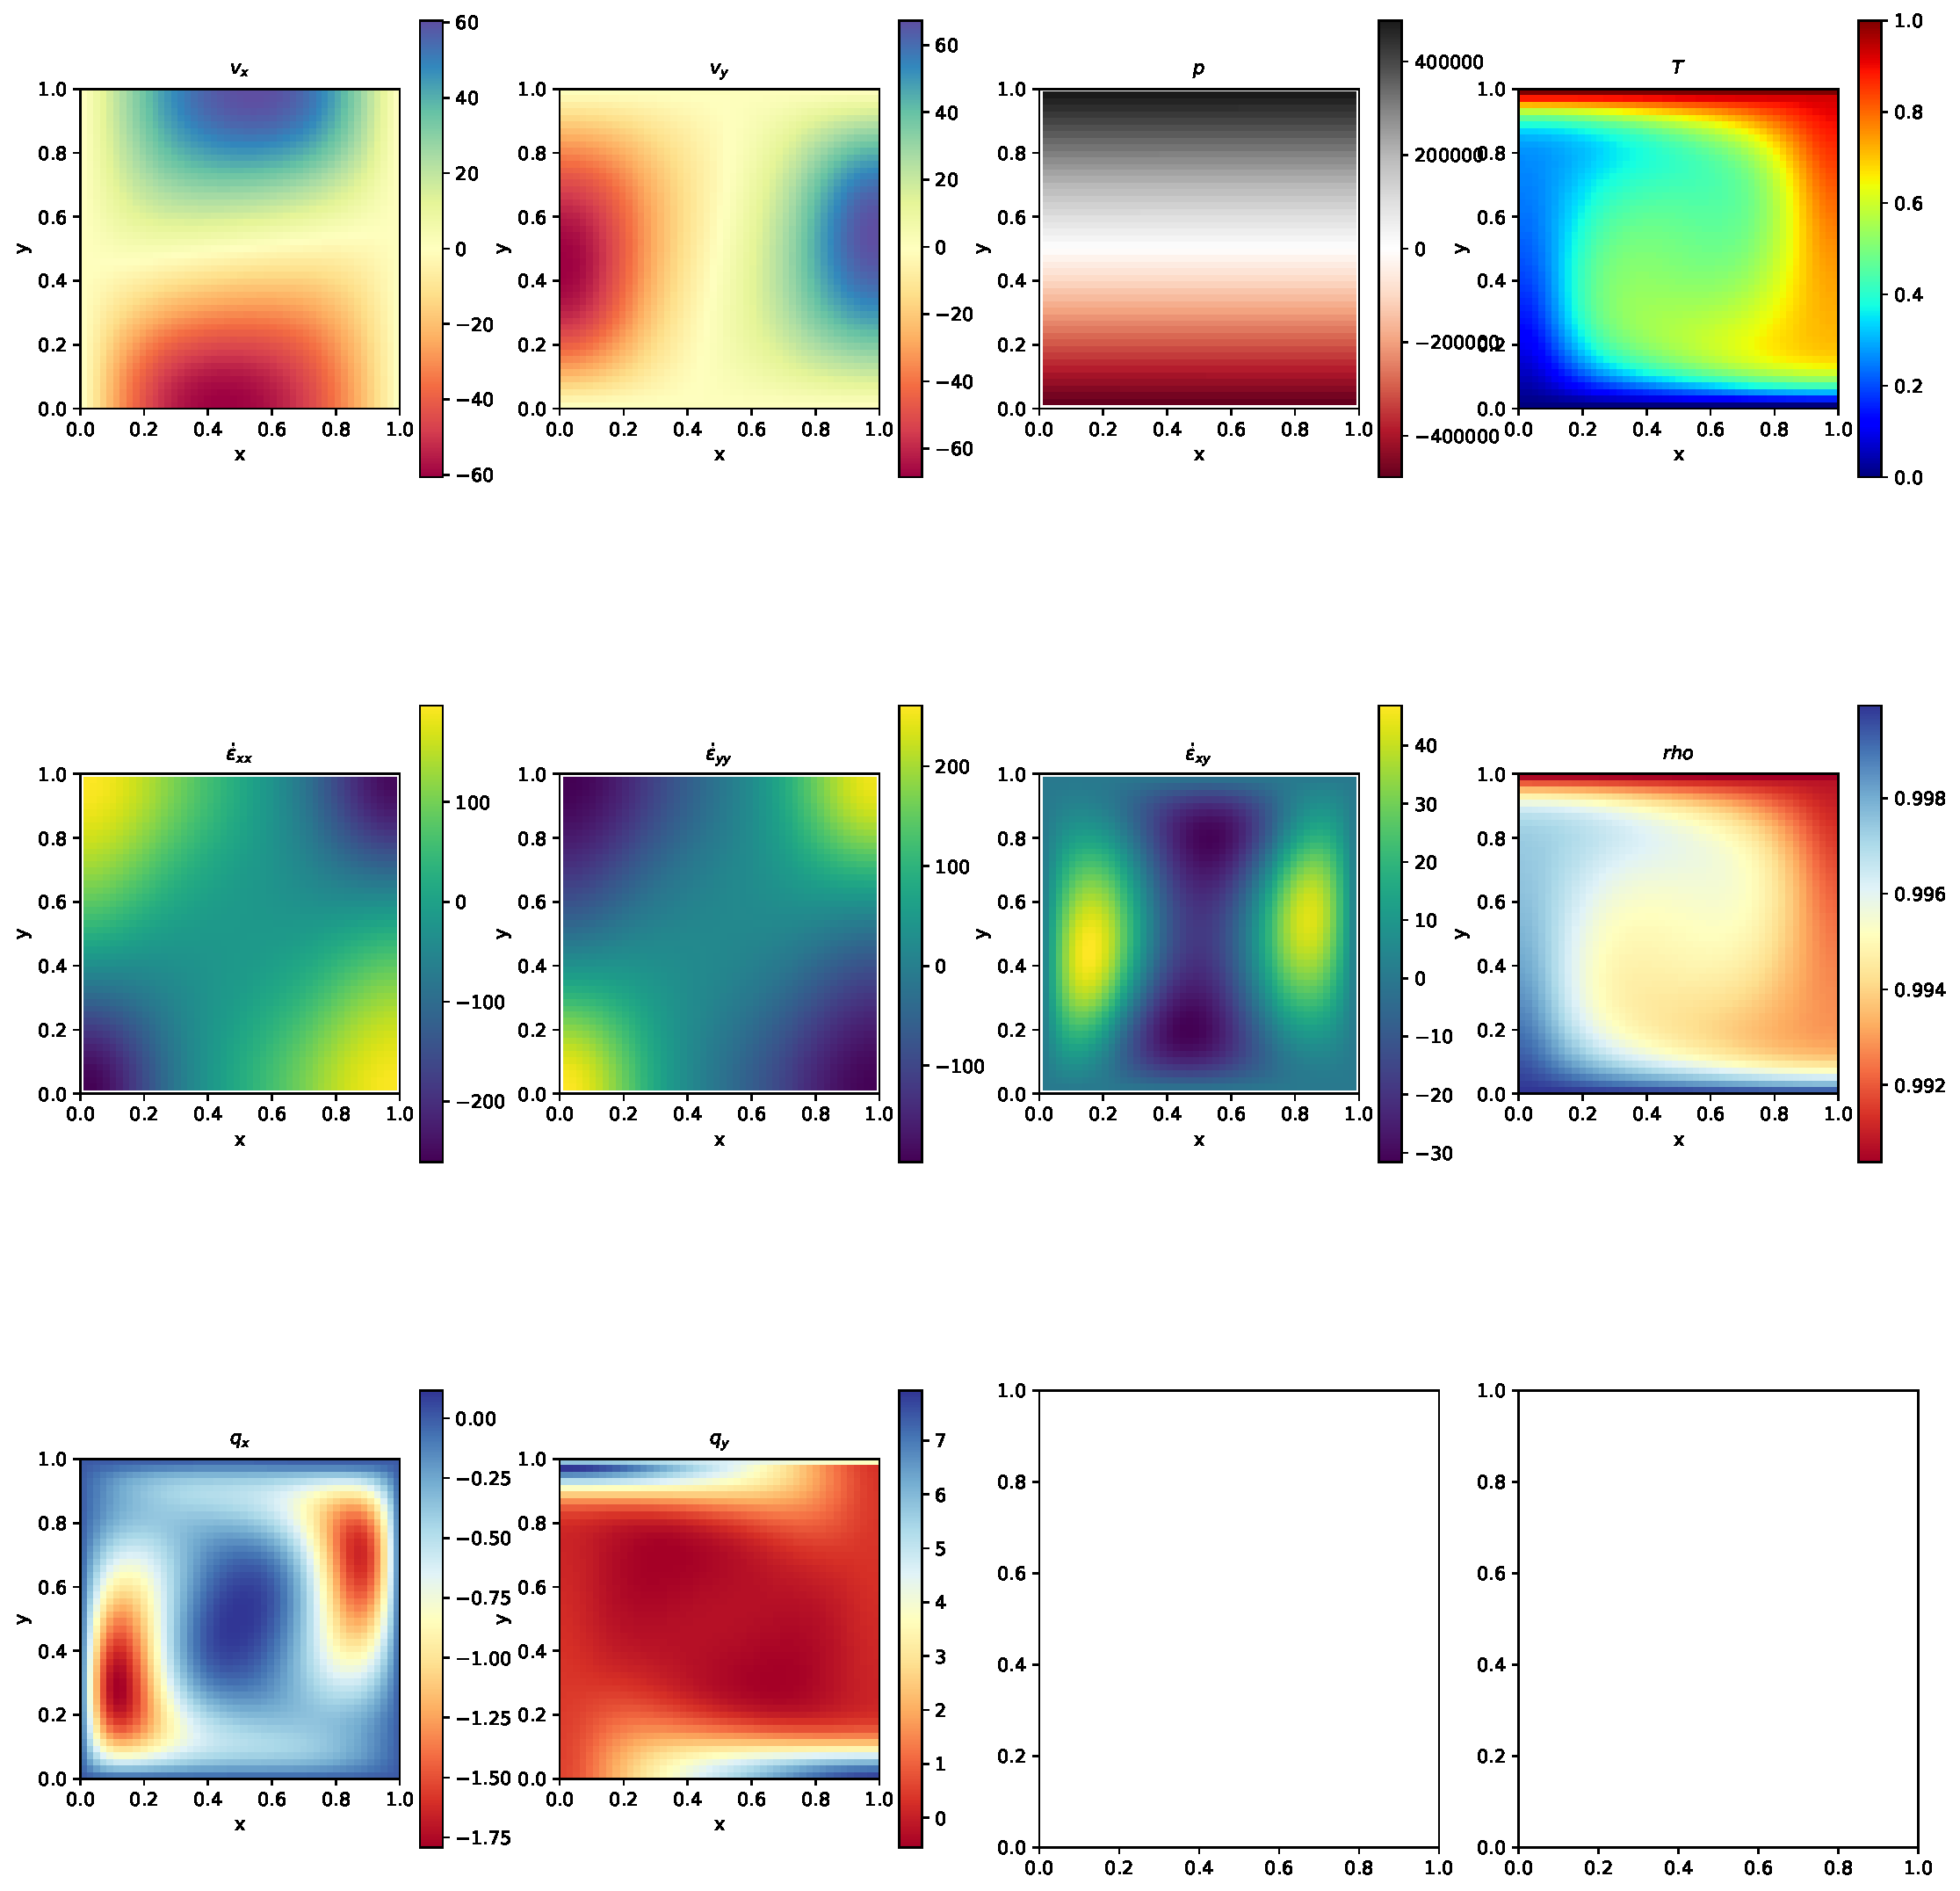
\includegraphics[width=16cm]{python_codes/fieldstone_03/results_1e4/48x48/solution.pdf}\\
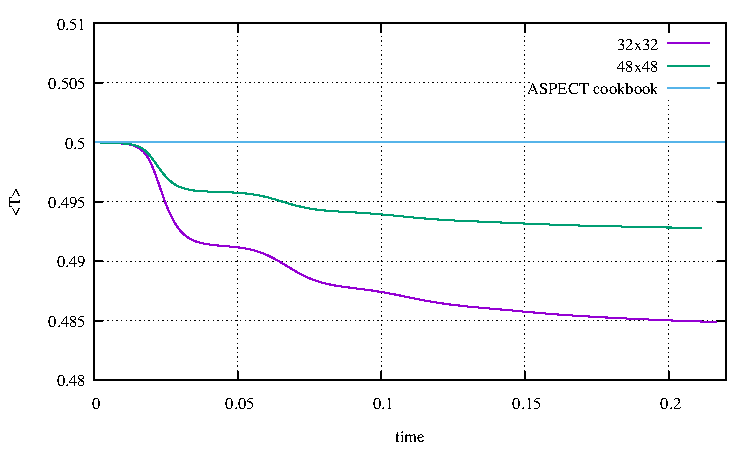
\includegraphics[width=5cm]{python_codes/fieldstone_03/results_1e4/Tavrg.pdf}
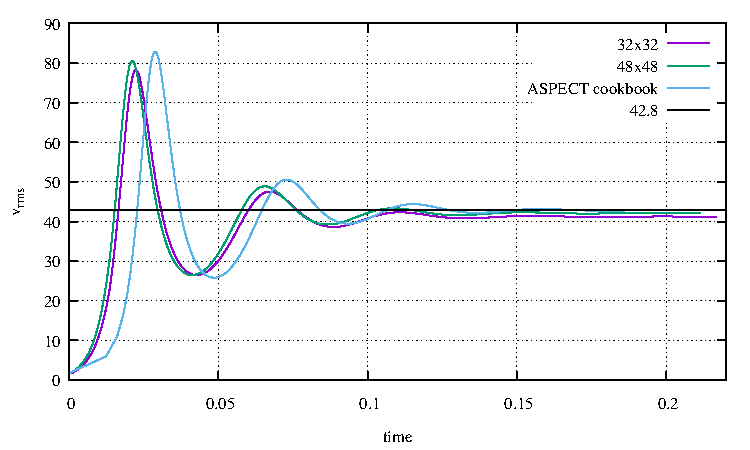
\includegraphics[width=5cm]{python_codes/fieldstone_03/results_1e4/vrms.pdf}\\
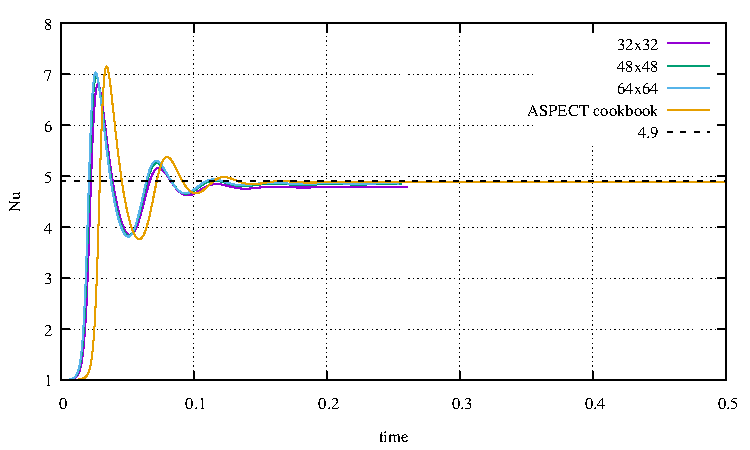
\includegraphics[width=5cm]{python_codes/fieldstone_03/results_1e4/Nu.pdf}
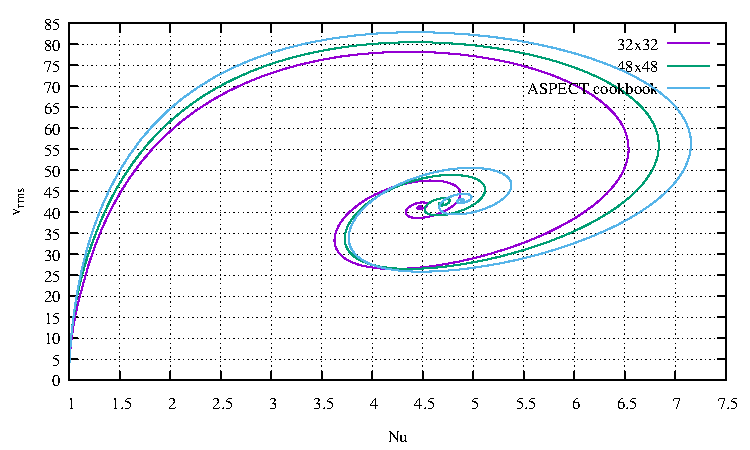
\includegraphics[width=5cm]{python_codes/fieldstone_03/results_1e4/Nu_vrms.pdf}
\end{center}

\newpage
\paragraph{Results for $\Ranb=10^5$}.
\begin{center}
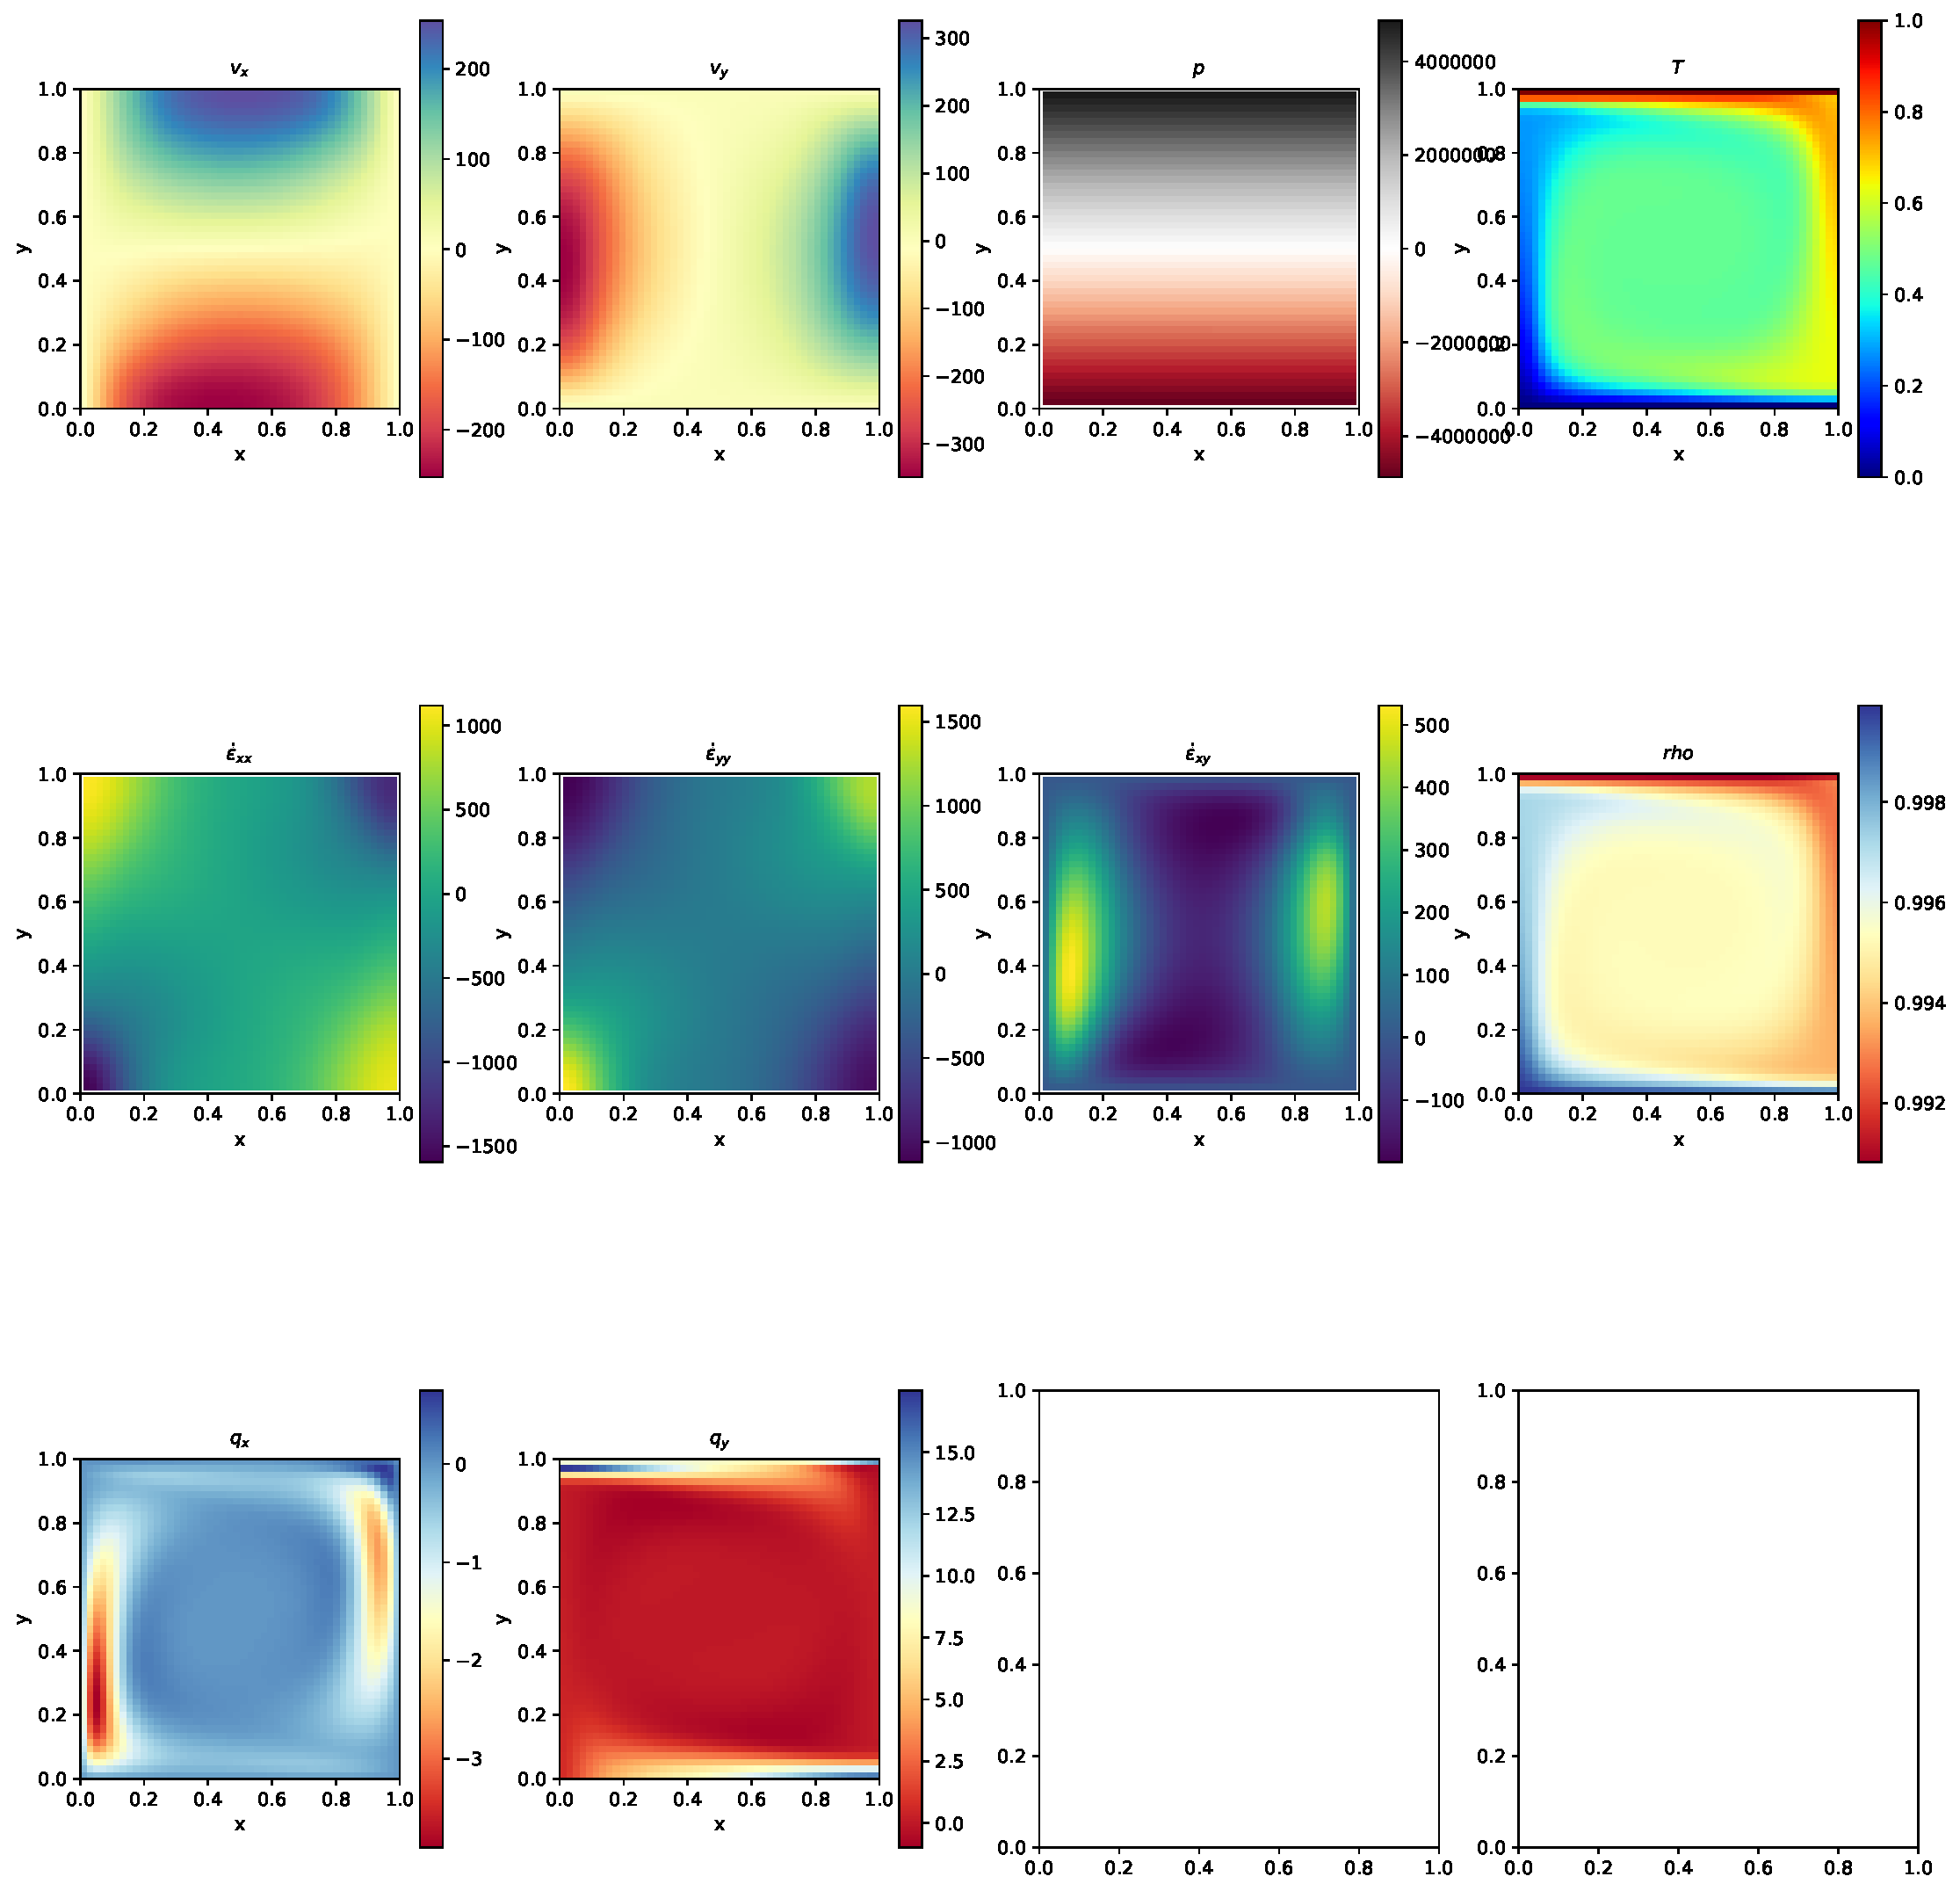
\includegraphics[width=16cm]{python_codes/fieldstone_03/results_1e5/48x48/solution.pdf}\\
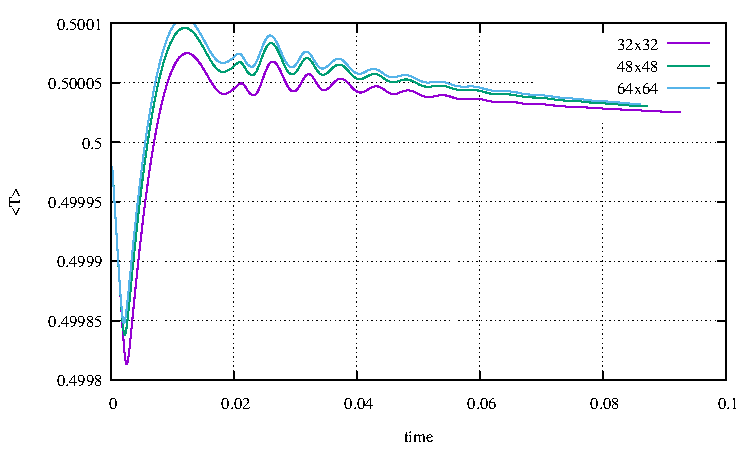
\includegraphics[width=5cm]{python_codes/fieldstone_03/results_1e5/Tavrg.pdf}
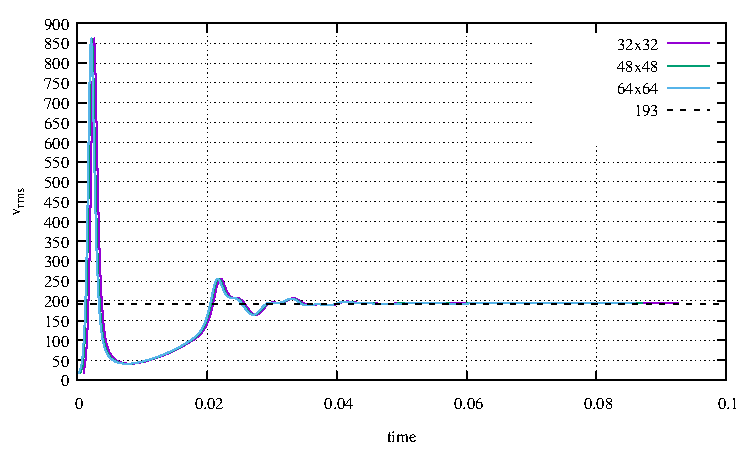
\includegraphics[width=5cm]{python_codes/fieldstone_03/results_1e5/vrms.pdf}\\
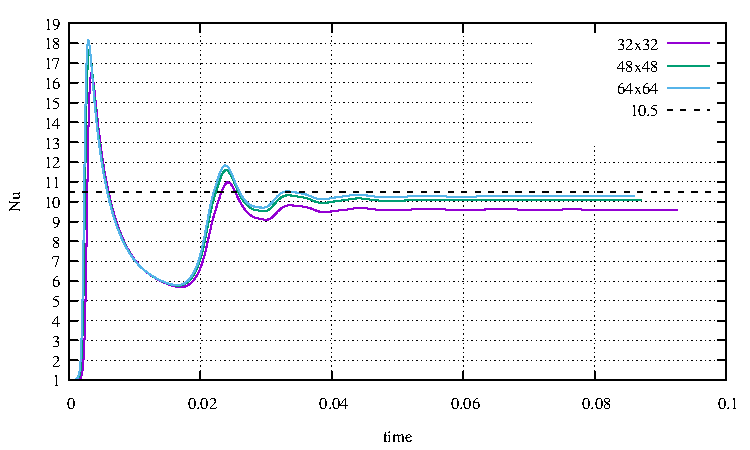
\includegraphics[width=5cm]{python_codes/fieldstone_03/results_1e5/Nu.pdf}
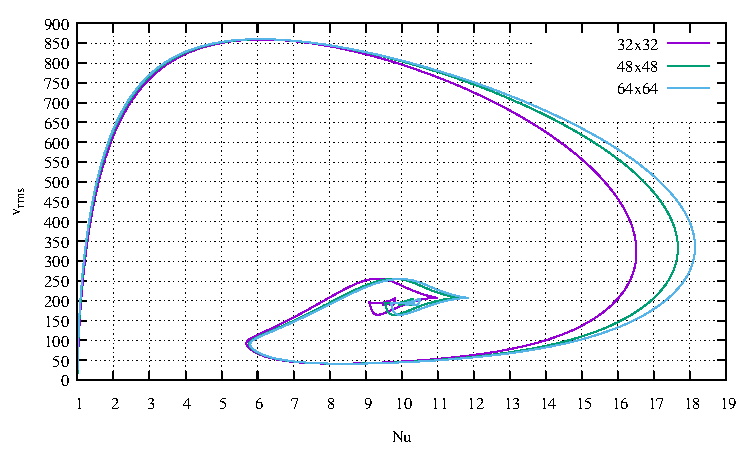
\includegraphics[width=5cm]{python_codes/fieldstone_03/results_1e5/Nu_vrms.pdf}
\end{center}

\newpage
\paragraph{Results for $\Ranb=10^6$}.
\begin{center}
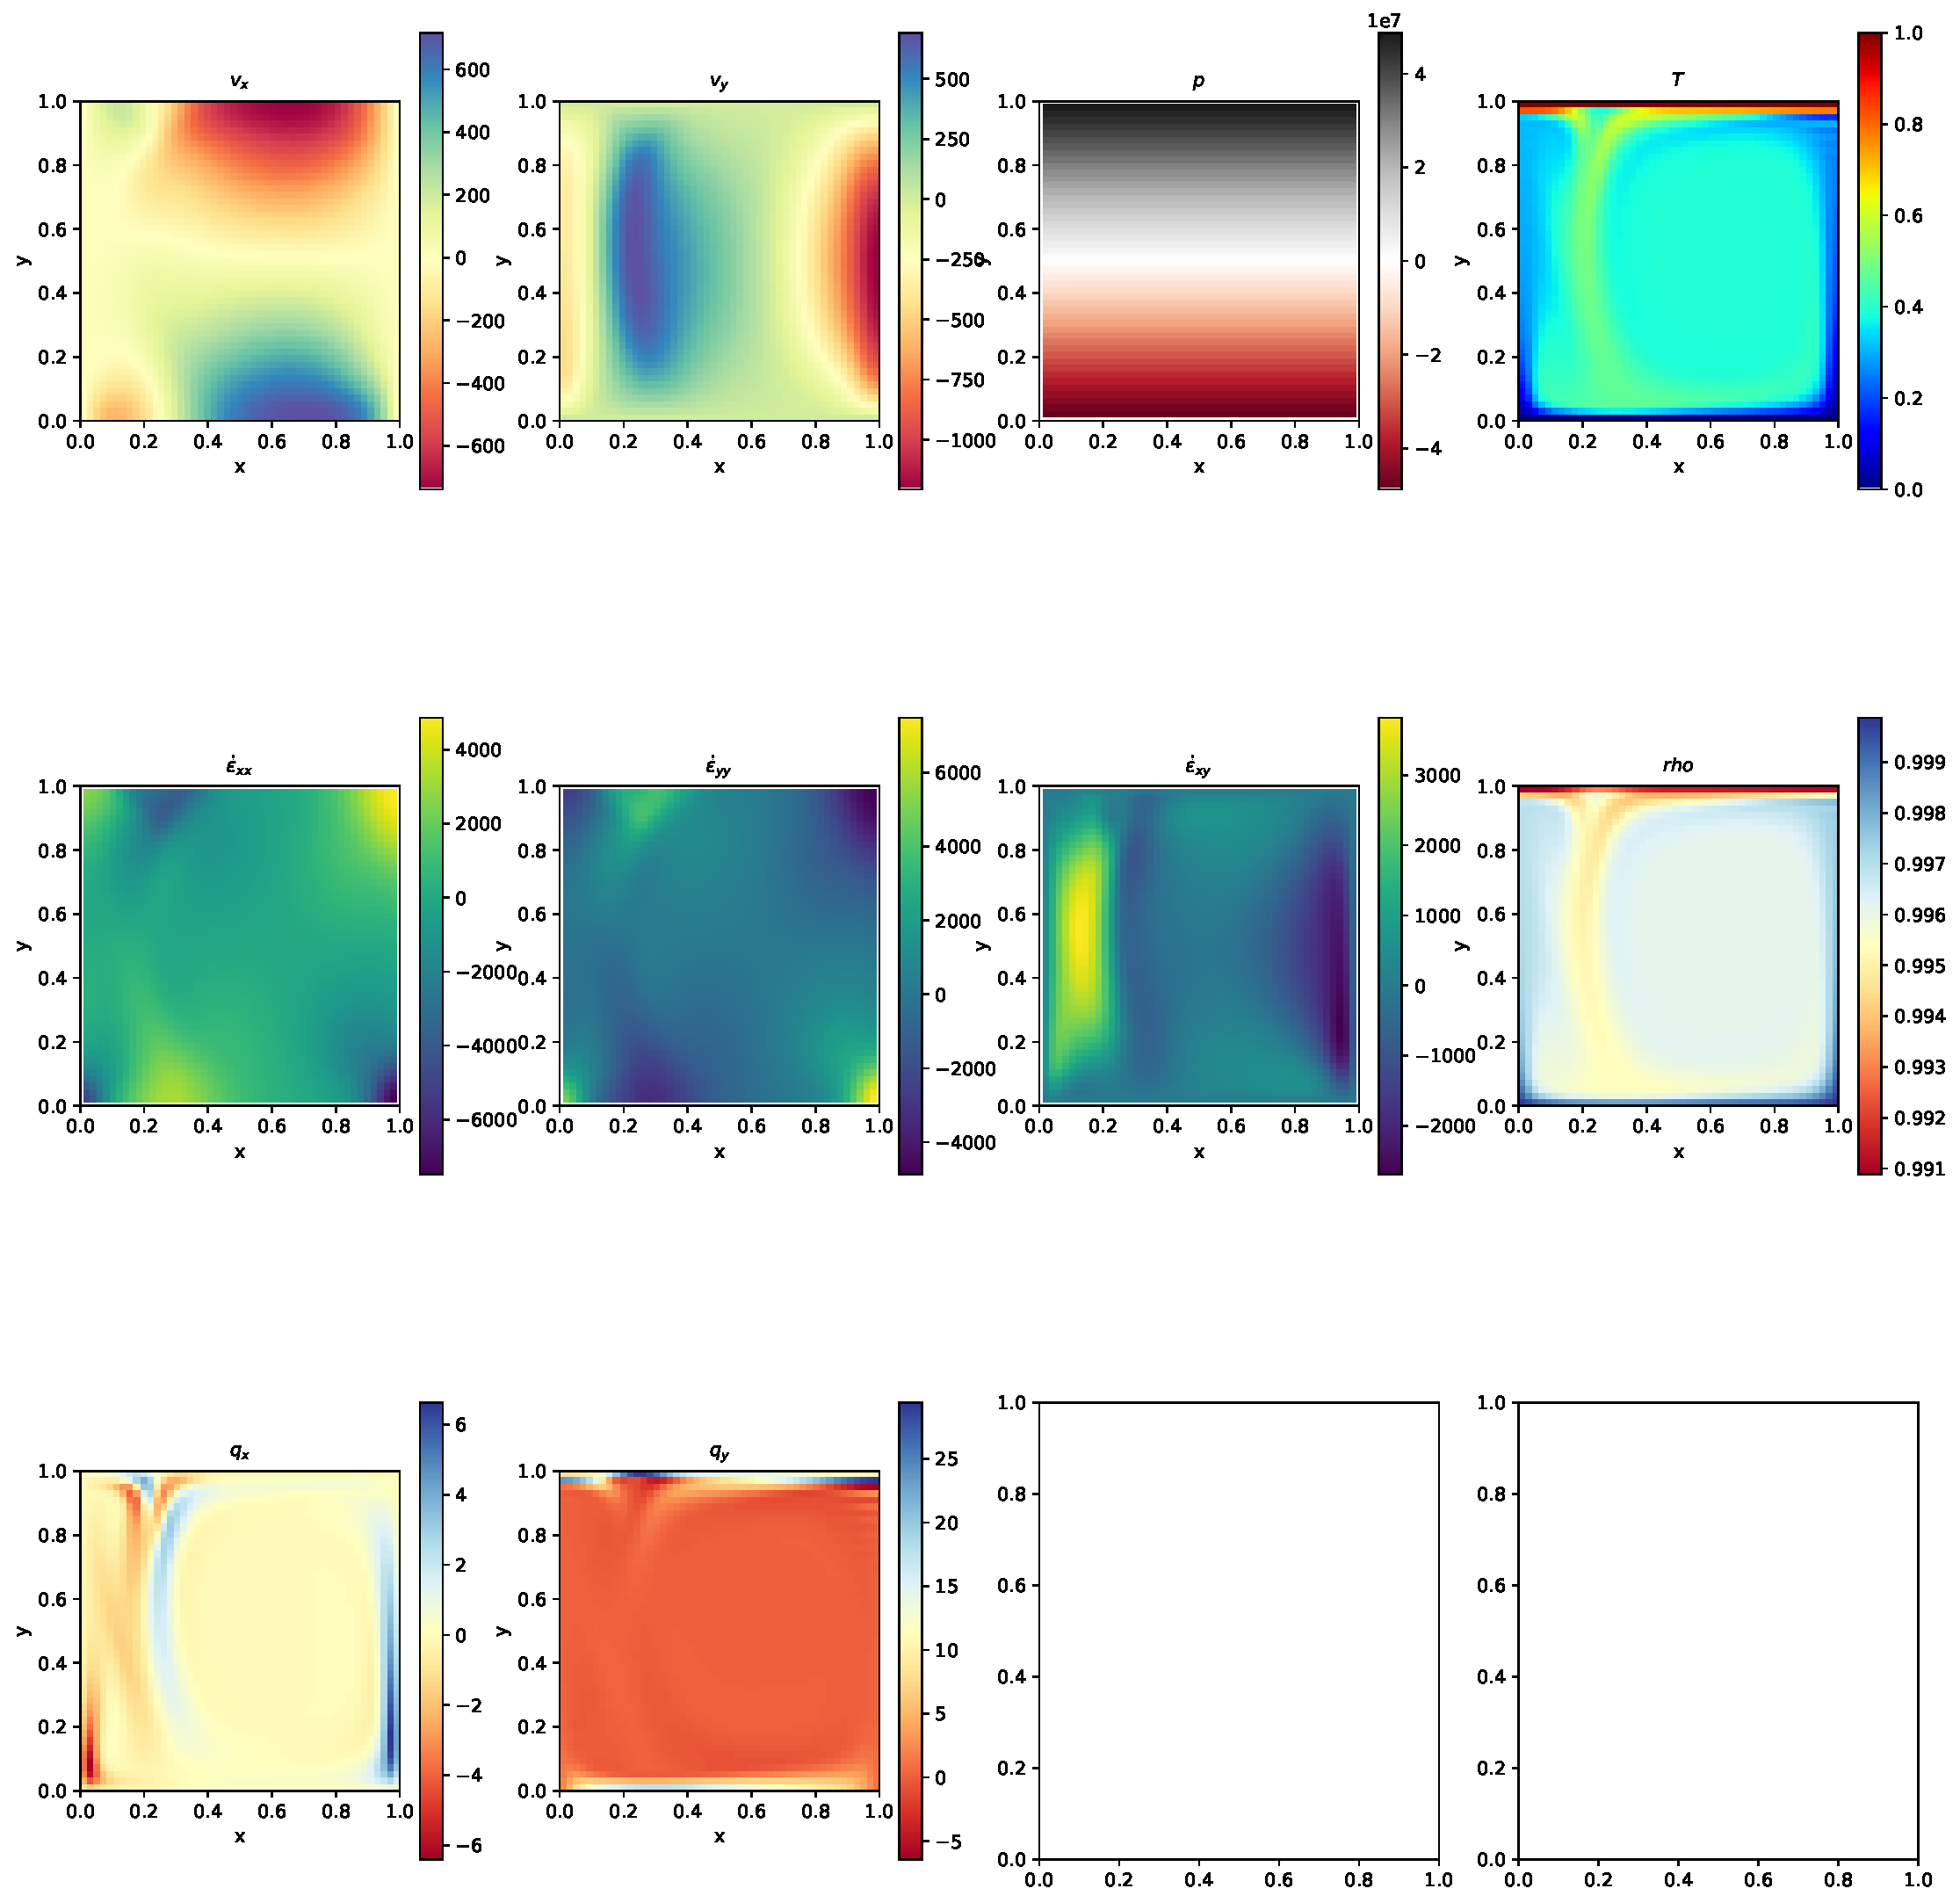
\includegraphics[width=16cm]{python_codes/fieldstone_03/results_1e6/48x48/solution.pdf}\\
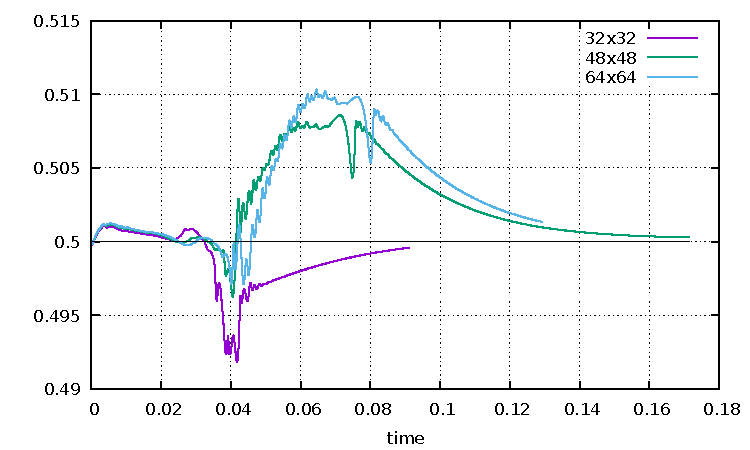
\includegraphics[width=5cm]{python_codes/fieldstone_03/results_1e6/Tavrg.pdf}
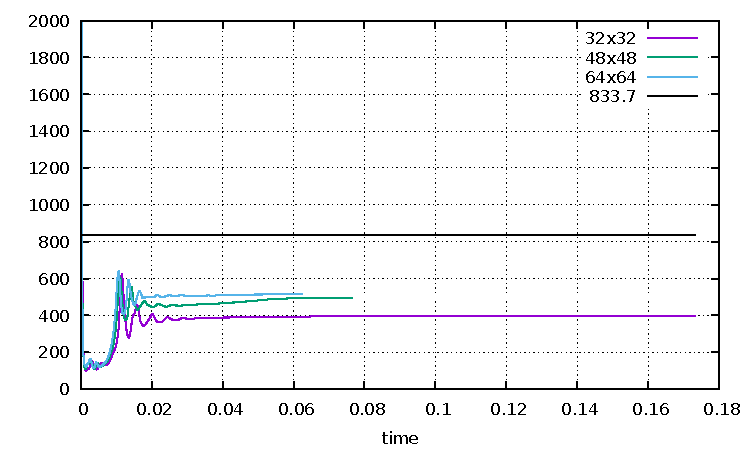
\includegraphics[width=5cm]{python_codes/fieldstone_03/results_1e6/vrms.pdf}\\
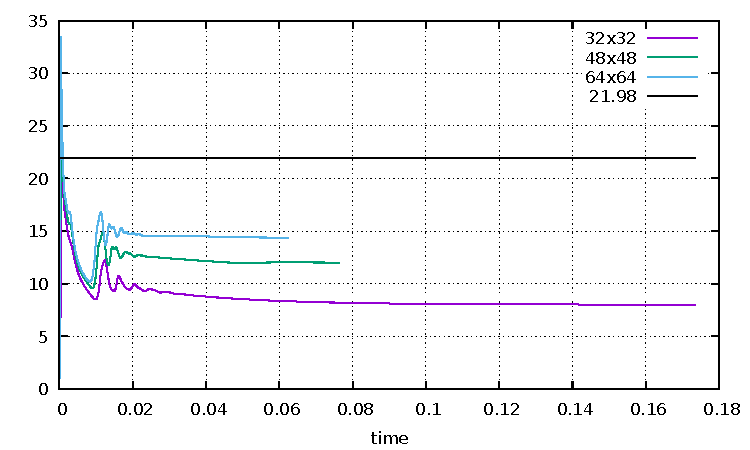
\includegraphics[width=5cm]{python_codes/fieldstone_03/results_1e6/Nu.pdf}
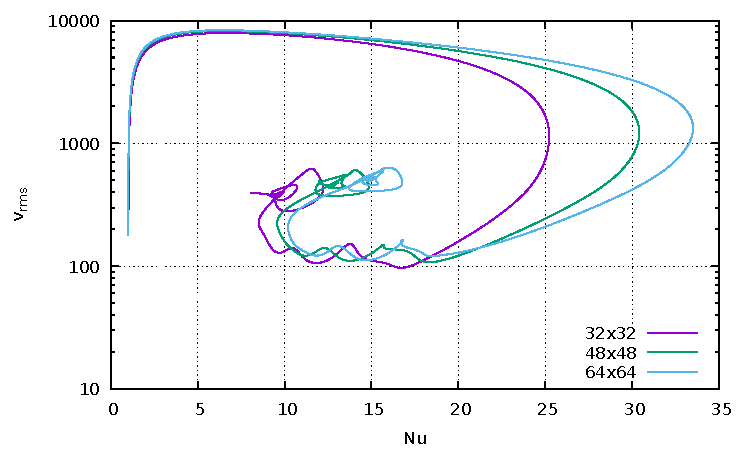
\includegraphics[width=5cm]{python_codes/fieldstone_03/results_1e6/Nu_vrms.pdf}
\end{center}


I have tested the influence of the CFL number (0.5 instead of 1) and it does not change much at all.





